
%\documentclass[conference]{IEEEtran}
\documentclass[10pt, conference, compsocconf]{IEEEtran}

% \hyphenation{op-tical net-works semi-conduc-tor}
\usepackage{graphicx}
%\usepackage[square, numbers, comma, sort&compress]{natbib}
%\usepackage{verbatim} 
%\usepackage{vector}
%\usepackage{amsthm}
%\usepackage{array}
%\usepackage{tabularx}
%\usepackage{multirow}
%\usepackage{fixltx2e}
%\usepackage[english]{babel}
%\usepackage{amsmath}
%\usepackage{todonotes}
%\usepackage[]{algorithm2e}
%\usepackage{pgfplots}
%\usepackage[justification=centering,font=small]{caption}
%\usepackage{url}
%\usepackage{pdfpages}

\begin{document}
%\title{An Efficient Approach for Mining Frequent Patterns over Uncertain Data Stream}
\title{An Efficient Approach for Mining Frequent Patterns over Uncertain Data Streams}

%\author{
%    \IEEEauthorblockN{Md. Badi-Uz-Zaman Shajib\IEEEauthorrefmark{1}, Md. Samiullah\IEEEauthorrefmark{1}, Chowdhury Farhan Ahmed\IEEEauthorrefmark{1}, Carson Kai-Sang Leung\IEEEauthorrefmark{2}}
%    \IEEEauthorblockA{\IEEEauthorrefmark{1}Department of Computer Science \& Engineering, University of Dhaka, Bangladesh
%    \\mbzshajib@gmail.com, samiullah@cse.univdhaka.edu, farhan@du.ac.bd}
%    \IEEEauthorblockA{\IEEEauthorrefmark{3}Department of Computer Science University of Manitoba, Canada
%    \\kleung@cs.manitoba.ca}
%}

\author{\IEEEauthorblockN{Md. Badi-Uz-Zaman Shajib ~ Md. Samiullah ~ Chowdhury Farhan Ahmed}
\IEEEauthorblockA{Department of Computer Science and Engineering\\
University of Dhaka\\
Dhaka, Bangladesh\\
mbzshajib@gmail.com, samiullah@cse.univdhaka.edu, farhan@du.ac.bd}
\and
\IEEEauthorblockN{Carson K. Leung ~ Adam G.~M. Pazdor}
\IEEEauthorblockA{Department of Computer Science\\
University of Manitoba\\
Winnipeg, MB, Canada\\
\{kleung, umpazdor\}@cs.umanitoba.ca}
}

\maketitle

\begin{abstract}
Knowledge discovery in big data is one of most interesting topics in state-of-the-art research, and frequent patterns mining is a major task. With the rapid growth of modern technology, high volumes of data---which are of different veracities (i.e., may be precise or uncertain)---are flowing at a high velocity all over the world. Properties of data temporally changes with changes in the people's interests, which make the data dynamic. Due to the uncertainty and dynamic properties of data, finding appropriate and efficient approach to ensure the efficient usage of available resources has become a great challenge. In this paper, we design a new memory-efficient data structure, called {\em Uncertain Stream $($US$)$-tree}, which stores recent meta-data. We also develop a probabilistic, sliding window based, efficient algorithm---called {\em Uncertain Stream Frequent Pattern $($USFP$)$-growth}---for mining frequent patterns from uncertain data streams. Our comprehensive performance evaluation shows that USFP-growth is correct and efficient when compared with recent related approaches.\\[-5pt]

\textit{Keywords}---
%\end{abstract}
%\begin{IEEEkeywords}
Data mining; frequent pattern mining; uncertain data; data streams; sliding window
%\end{IEEEkeywords}
\end{abstract}

%\IEEEpeerreviewmaketitle

\section{Introduction and Related Work}\label{Related_work}

Knowledge discovery in databases (KDD) aims to extract efficient, helpful, functional and valuable information from very large databases and to use the extracted valuable information in different applications (e.g., automated analysis, business, research). In recent years, with increases of modern technologies and popularity of Internet, high volumes of data are produced.
In the current era of big data, devices like smart-phones, smart-gears (e.g., smart watches, smart glasses) are collecting data at a high velocity (e.g., every micro second) but of different veracities (e.g., imprecise meteorological data like $-$30$\pm$3$^\circ$C).
Data uncertainty is an inherent property in various applications due to reasons such as hardware fault, uncertainty of incidents, outdated sources, and imprecise/incorrect measurements. These big data are constantly growing in volume, variety, velocity, and uncertainty. Temporal-spatial data collected by GPS-enabled tracking devices, meteorological data collected by weather instruments or sensors, biological or medical data collected by sensors are examples of uncertain data.

Over the past decade, many algorithms have been developed for mining frequent itemsets or patterns from uncertain data. Among them, many were designed based on either Apriori~\cite{DBLP:conf/vldb/AgrawalS94} or FP-growth~\cite{DBLP:journals/datamine/HanPYM04} algorithms. 
For instance, \mbox{U-Apriori}~\cite{DBLP:journals/tkde/ZhaoYN14} is an Apriori-based candidate generate-and-test algorithm for mining frequent patterns from uncertain data.
While UF-growth~\cite{DBLP:conf/kdd/GadeWK04} and UFP-growth~\cite{DBLP:conf/kdd/AggarwalLWW09} are tree-based algorithms, their tree are not too compact.
\mbox{PUF-growth}~\cite{DBLP:conf/pakdd/LeungT13} improves the situations by constructing more compact (PUF-)trees at a price of producing a few false positives.

As big data can be generated at a high velocity, frequent pattern mining algorithms for mining data streams were developed. For instance, UF-streaming~\cite{DBLP:conf/icde/LeungH09} and \mbox{SUF-growth}~\cite{DBLP:conf/icde/LeungH09} were proposed to mine uncertain frequent pattern from streams. 
However, as an approximate algorithm, \mbox{UF-streaming}~\cite{DBLP:conf/icde/LeungH09} may produce both false positives and false negatives. As an exact algorithm, SUF-growth~\cite{DBLP:conf/icde/LeungH09} resolves the problem of the generation of false positives and false negatives but at a potential price of constructing bushy trees.
To elaborate, 
UF-streaming~\cite{DBLP:conf/icde/LeungH09} is a sliding window-based algorithm, which captures most recent data. To mine frequent patterns, the algorithm divides the transactions in the data streams into several batches. Once the transactions in each batch are inserted into the UF-tree structure~\cite{DBLP:conf/kdd/GadeWK04}, UF-streaming then calls \mbox{UF-growth}~\cite{DBLP:conf/kdd/GadeWK04} to mine each \mbox{UF-tree} for frequent patterns, which are  subsequently stored in a UF-stream structure. To avoid false negatives, UF-streaming uses a {\it preMinSup} threshold, which is less than the usual user-specified minimum support {\it minsup} threshold (i.e., $0 < {\it preMinSup} \leq {\it minsup}$). 
When data streams flow, the window slides, frequent patterns mined from older batches are then removed from the UF-stream structure and frequent patterns mined from newer batches are inserted into the UF-stream structure. Hence, a potential problem is that, if one wants to obtain frequent patterns after the 50th batch when using a sliding window of size 3, unnecessary mining is needed to be performed on the first 47~batches.
To address this potential problem, SUF-growth~\cite{DBLP:conf/icde/LeungH09} returns only truly frequent patterns by using a delayed mode for mining. As a result, unnecessary computation is reduced, and unnecessary mining is avoided. Specifically, the algorithm divides the transactions in the data streams into several batches. Once the transactions in each batch are inserted into a \mbox{SUF-tree} structure, which is similar to the UF-tree structure but is designed for processing batches of transactions in data streams with the slidling window model. When data streams flow, the window slides, transactions in older batches are then removed from the SUF-tree structure and transactions in newer batches are inserted into the SUF-tree structure. In other words, instead of keeping mining the tree structure for frequent patterns, SUF-growth keeps updating the tree structure and mines the updated tree structure when needed. Hence, if one wants to obtain frequent patterns after the 50th batch when using a sliding window of size 3, no unnecessary mining is needed to be performed on the first 47~batches. Mining is performed after the 50th updates. However, inherited from UF-trees, SUF-trees can be bushy. 
This motivates our work in this paper: We propose a probabilistic sliding window based efficient and optimized approach for handling uncertain data stream.
{\em Our contributions of this paper} are as follow:
Our key contributions of this paper are as follow:
\begin{itemize}
  \item For each item in a transaction, we introduce a prefix value---denoted as $U^{cap}$---that maintains an upper bound of probability. Such a bound helps to construct a compact pattern tree.
  \item We design a new data-structure called \emph{Uncertain Stream $($US$)$-tree}, which is compact,  is memory-efficient, and follow the partial downward closure property.
  \item We develop a new mining algorithm called \emph{Uncertain Stream Frequent Pattern $($USFP$)$-growth} algorithm, which significantly reduces mining time.
  \item We demonstrate the applicability and practicality (in terms of runtime, memory efficiency, and scalability) of the proposed algorithm in wide range of applicable areas
  \end{itemize}
The remainder of this paper is as follow. The next section provides the details of our proposed algorithm. Experimental results with comparison and analysis are given in Section~\ref{Experiment}. Section~\ref{Conclusion} presents the conclusions.

\section{Our Proposed Approach}\label{proposedWork}

To deal with stream property, we propose a sliding window-based algorithm---called {\em Uncertain Stream Frequent Pattern $($USFP$)$-growth}---with which we keep the most recent information. For uncertain data streams, each item in different transactions may have a different existential probability. Hence, it may become very difficult to merge (share) these paths in the corresponding tree structure. This uncertainty property of items may make the tree unmanageable and large. We also propose a new $U^{cap}$ value for each item that helps to share a single node in the {\em Uncertain Stream $($US$)$-tree}.  The US-tree structure is compact, and the USFP-growth is efficient for mining frequent patterns and removing false positives.

\subsubsection{Preliminaries about $U^{cap}$}

As an upper bound to the expected support, the $U^{cap}$ value can be computed as follows:
    \begin{equation}\label{equation:cap}
	U^{cap}(x_r) = \left\{
	\begin{array}{ll}
		P(x_1) & \mbox{if $h$=1}\\
		M \times P(x_r) & \mbox{if $h$$>$1}
	\end{array}\right.
\end{equation}
where $M=\max_{1\leq q\leq h} P(x_q)$.
For the transaction $t_1 = \{a$:0.9, $c$:0.6, $d$:0.5, $e$:0.2\}, 
$U^{cap}(a) = 0.9$ because $a$ is the first item in the prefix. 
$U^{cap}(c) = 0.9 \times 0.6 = 0.54$ because $a$ (with existence probability 0.9) is the only item preceding $c$. 
$U^{cap}(d) = 0.9 \times 0.5 = 0.45$ because $a$ has the highest existence probability between the two items (namely, $a$ and $c$) preceding $d$.
Similarly, $U^{cap}(e) = 0.9 \times 0.2 = 0.18$ because $a$ has the highest existence probability among the three items (namely, $a, c$ and $d$) preceding $e$.
Note that, as an upper bound, the existential probability of any items is no more than $U^{cap}$; i.e., $\forall(i,j) \{P(I_i) \times P(I_j)\leq U_{cap}(I_j)\}$, where $i < j$.
As a pattern with $U^{cap} < {\it minsup}$ is guaranteed to be infrequent, no false negative is generated.
So, our proposed USFP-growth algorithm can be divided into five key steps:
(1) Group transactions into different batches of the window size, and compute $U^{cap}$;
(2) Insert transactions into the US-tree structure;
(3) Slide windows within the US-tree structure;
(4) Mine frequent patterns from the US-tree; and
(5) Eliminate false positive.

\subsubsection{Preparation}\label{sec:prep}

%%\documentclass{article} 
%\usepackage{graphicx}  
%\usepackage{multirow}
%\usepackage[table]{xcolor}
%\usepackage{fixltx2e}
%\usepackage{array}
%
%\begin{document}
\begin{table}
\centering

\begin{tabular}{|c|c|c|c|c|c|}
\hline
	Batch No& Transaction No & \multicolumn{4}{c|}{Items in Transaction} \\ \hline \hline
	\multirow{3}{*}{Batch 1}	&	T\textsubscript{1} & a(0.9) & c(0.54) & d(0.45) & e(0.18)		\\
								&	T\textsubscript{2} & a(0.9) & b(0.36) & e(0.09) & --			\\
								&	T\textsubscript{3} & a(0.2) & c(0.18) & d(0.63) & --			\\\hline
	\multirow{3}{*}{Batch 2}	&	T\textsubscript{4} & b(0.3) & c(0.27) & --  	& --			\\
								&	T\textsubscript{5} & a(0.1) & b(0.03) & c(0.27) & --  			\\
								&	T\textsubscript{6} & a(0.9) & e(0.27) & --	    & --  			\\\hline
	\multirow{3}{*}{Batch 3}	&	T\textsubscript{7} & a(0.1) & d(0.06) & e(0.12) & --			\\
								&	T\textsubscript{8} & a(0.1) & c(0.02) & f(0.12) & --   			\\
								&	T\textsubscript{9} & c(0.2) & d(0.09) & f(0.54) & --   			\\\hline
								
	\multirow{3}{*}{Batch 4}	&	T\textsubscript{10} &  --  &  --  &  --  & --    				\\
								&	T\textsubscript{11} &  --  &  --  &  --  & --    				\\
								&	T\textsubscript{12} &  --  &  --  &  --  & --    				\\\hline
	\end{tabular}
\caption{Window and Batch of Table \ref{table:uncertain_stream_transaction}}
\label{table:prefix_assigned}
\end{table}


%
%\end{document}
Let batch size = 3~transactions and sliding window size = 2~batches. Then, the first batch $B_1$ consists of transactions $T_1, T_2$ \& $T_3$. Similarly, the second batch $B_2$ consists of transactions $T_4, T_5$ \& $T_6$; the third batch $B_3$ consists of transactions $T_7, T_8$ \& $T_9$. See Table~\ref{table:prefix_assigned}.
After processing the first two batches, the sliding window is full. So, when the data stream flows, the window slides, transactions from Batch~$B_1$ need to be removed from the tree (which captures the contents of transactions) before transaction from Batch~$B_3$ can be inserted into the tree.

\begin{table}[t]
\centering
\caption{An example of uncertain streaming transactions (which are grouped by batches) with their $U^{cap}$ values}
\label{table:prefix_assigned}
\vspace*{-3mm}
\begin{tabular}{ll}
\hline
%	Batch\# & Transaction ID & {Contents of transaction} \\ \hline
Transaction & $U^{cap}$\\ \hline
\multicolumn{2}{l}{Batch $B_1$:}\\
	$T_1 = \{a$:0.9, $c$:0.6, $d$:0.5, $e$:0.2\} & \{$a$:0.9, $c$:0.54, $d$:0.45, $e$:0.18\}\\
	$T_2 = \{a$:0.9, $b$:0.4, $e$:0.1\} & \{$a$:0.9, $b$:0.36, $e$:0.09\}\\
	$T_3 = \{a$:0.2, $c$:0.9, $d$:0.7\} & \{$a$:0.2, $c$:0.18, $d$:0.63\}\\
\hline
\multicolumn{2}{l}{Batch $B_2$:}\\
	$T_4 = \{b$:0.3, $c$:0.9\} & \{$b$:0.3, $c$:0.27\}\\
	$T_5 = \{a$:0.1, $b$:0.3, $c$:0.9\} & \{$a$:0.1, $b$:0.03, $c$:0.27\}\\
	$T_6 = \{a$:0.9, $e$:0.3\} & \{$a$:0.9, $e$:0.27\}\\
\hline
\multicolumn{2}{l}{Batch $B_3$:}\\
	$T_7 = \{a$:0.1, $d$:0.6, $e$:0.2\} & \{$a$:0.1, $d$:0.06, $e$:0.12\}\\
	$T_8 = \{a$:0.1, $c$:0.2, $f$:0.6\} & \{$a$:0.1, $c$:0.02, $f$:0.12\}\\
	$T_9 = \{c$:0.1, $d$:0.9, $f$:0.6\} & \{$c$:0.1, $d$:0.09, $f$:0.54\}\\
\hline
	\end{tabular}
\end{table}

\begin{figure*}[t]
    \begin{minipage}{0.45\linewidth}
        \centering
  		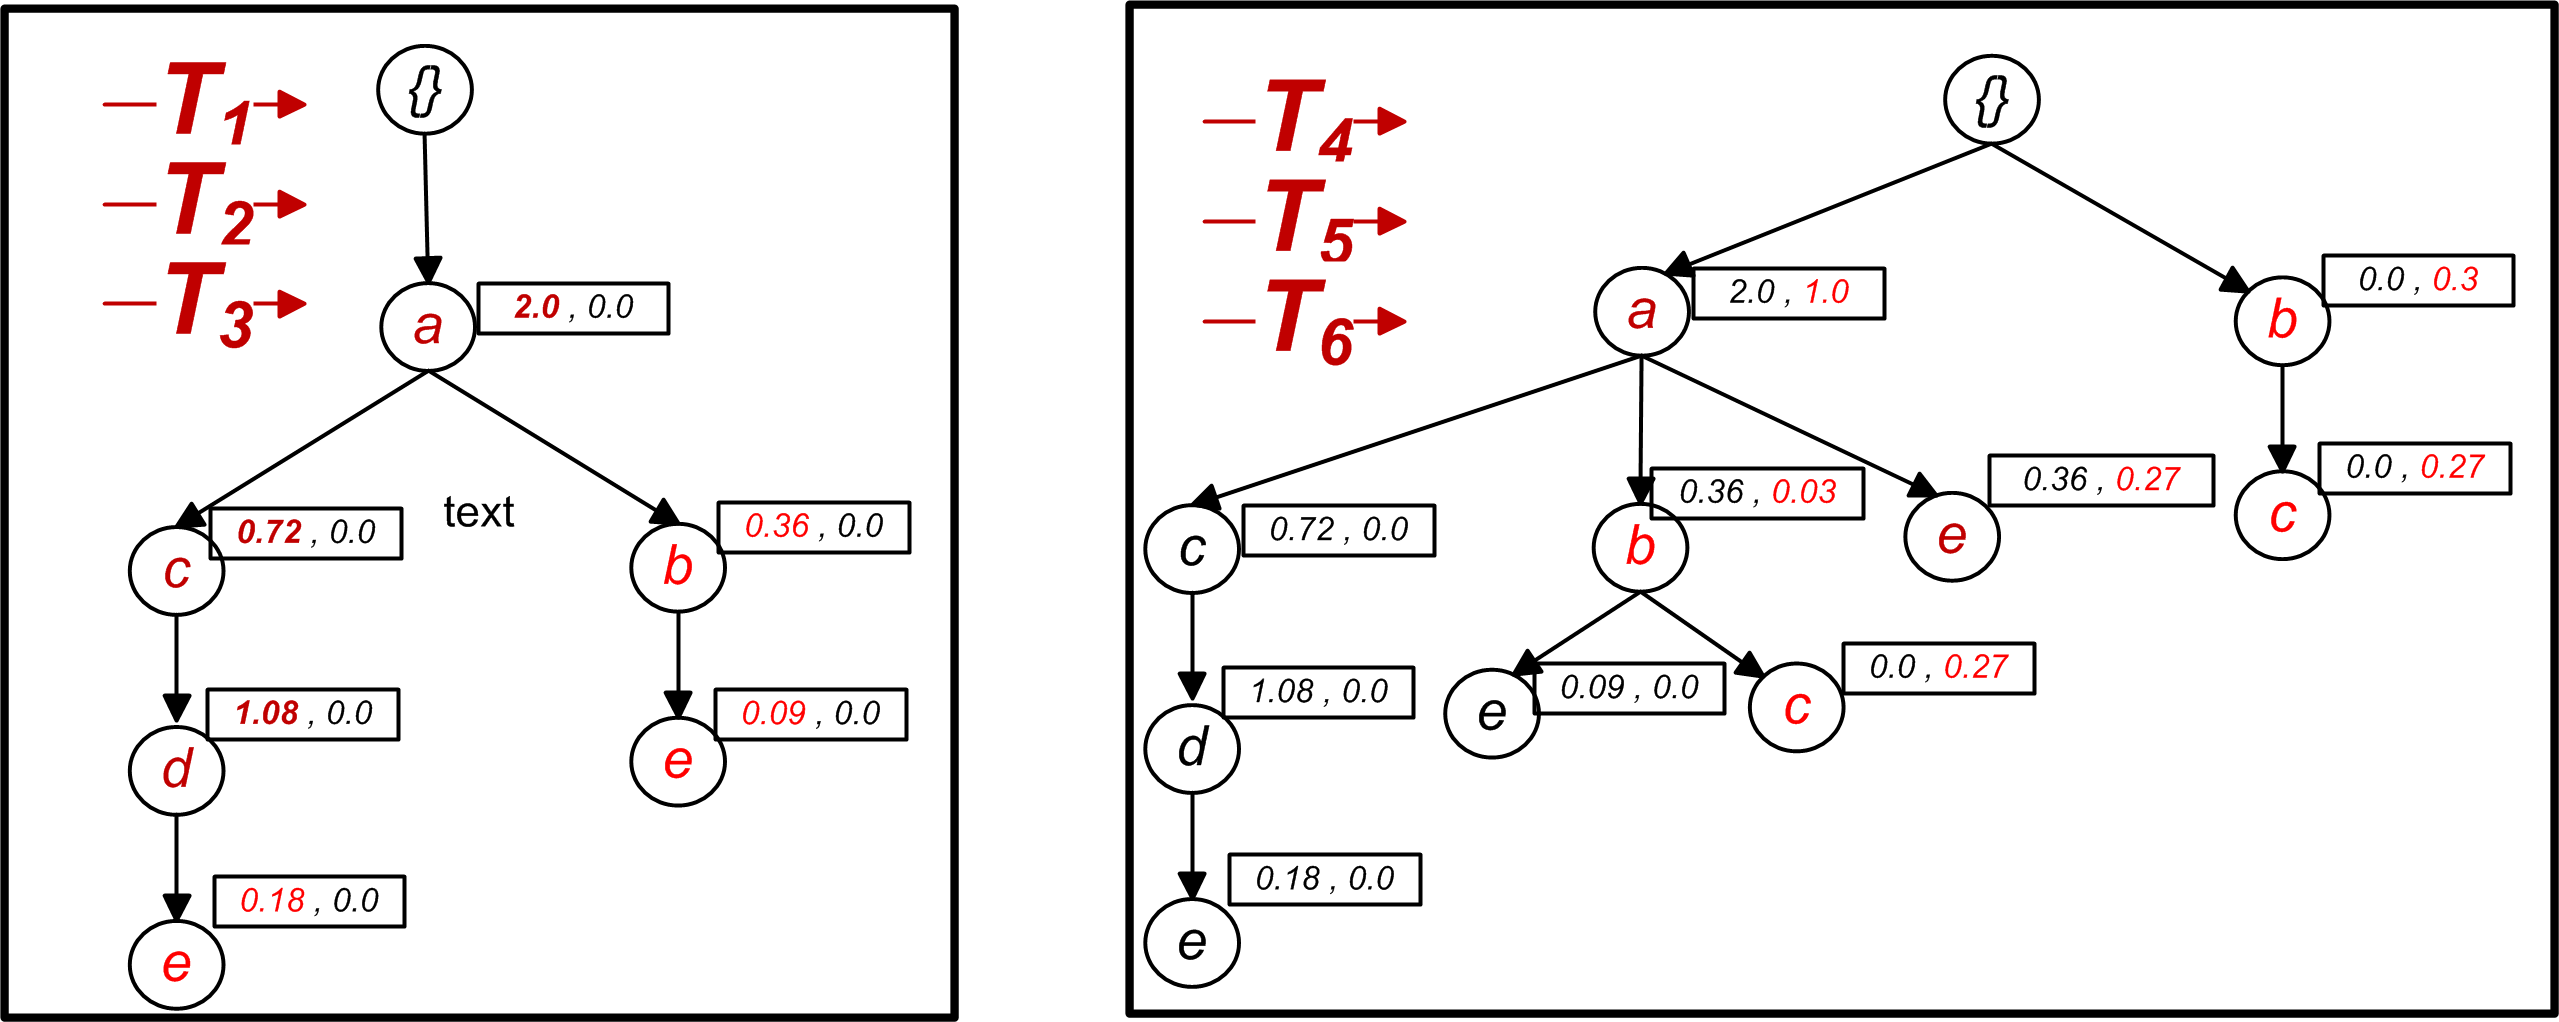
\includegraphics[width=0.9\textwidth]{visio/sim_1_6_V2}
		\vspace*{-3mm}
  		\caption{Constructing a US-tree.}
  		\label{figure:t1_6}
    \end{minipage}%	
    \begin{minipage}{0.55\linewidth}
         \centering
  		 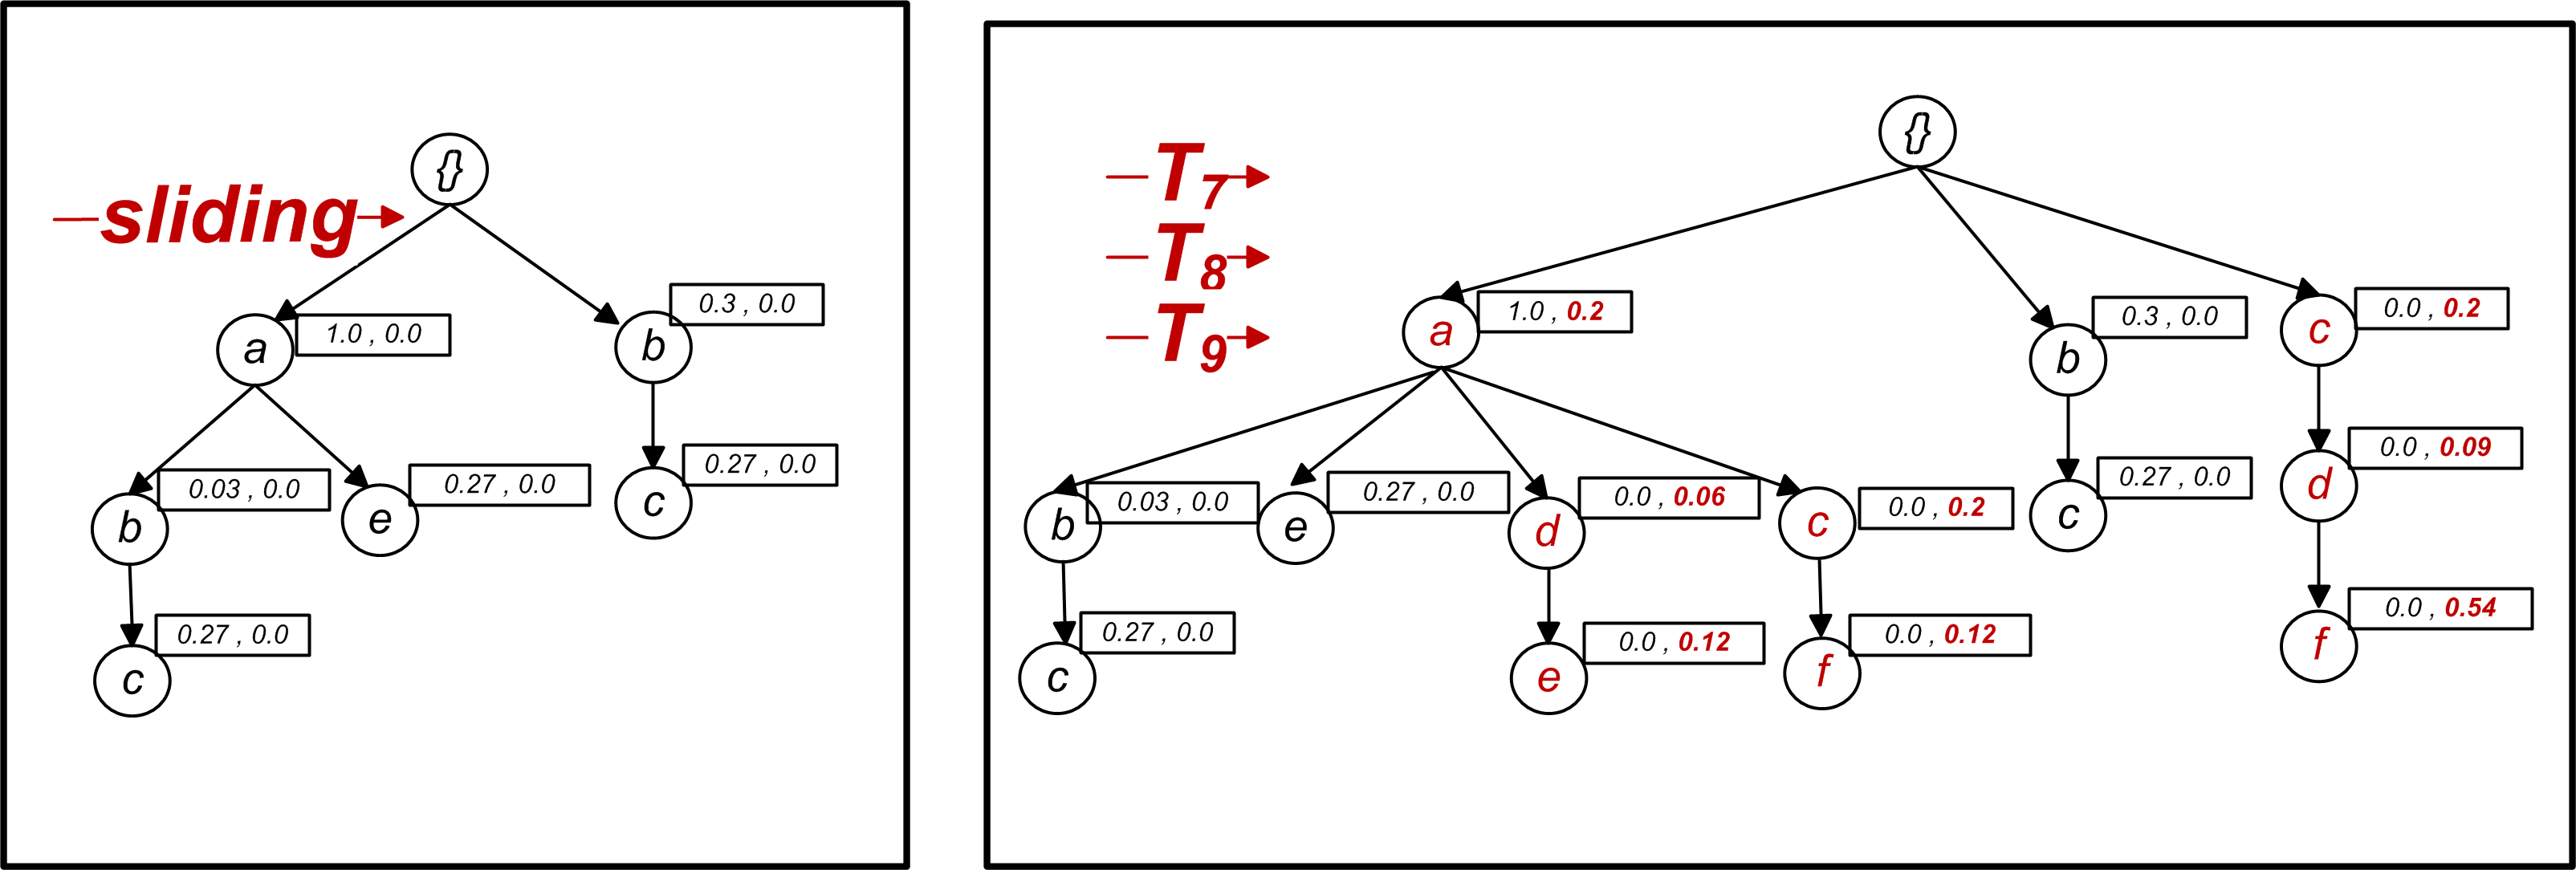
\includegraphics[width=0.9\textwidth]{visio/sim_06_slide_789_V2}
		\vspace*{-3mm}
  		 \caption{Updating the US-tree with a new sliding window.}
  		 \label{figure:t7_9}
    \end{minipage}	
\end{figure*}

\begin{figure*}[t]
    \begin{minipage}{0.45\linewidth}
	\centering
	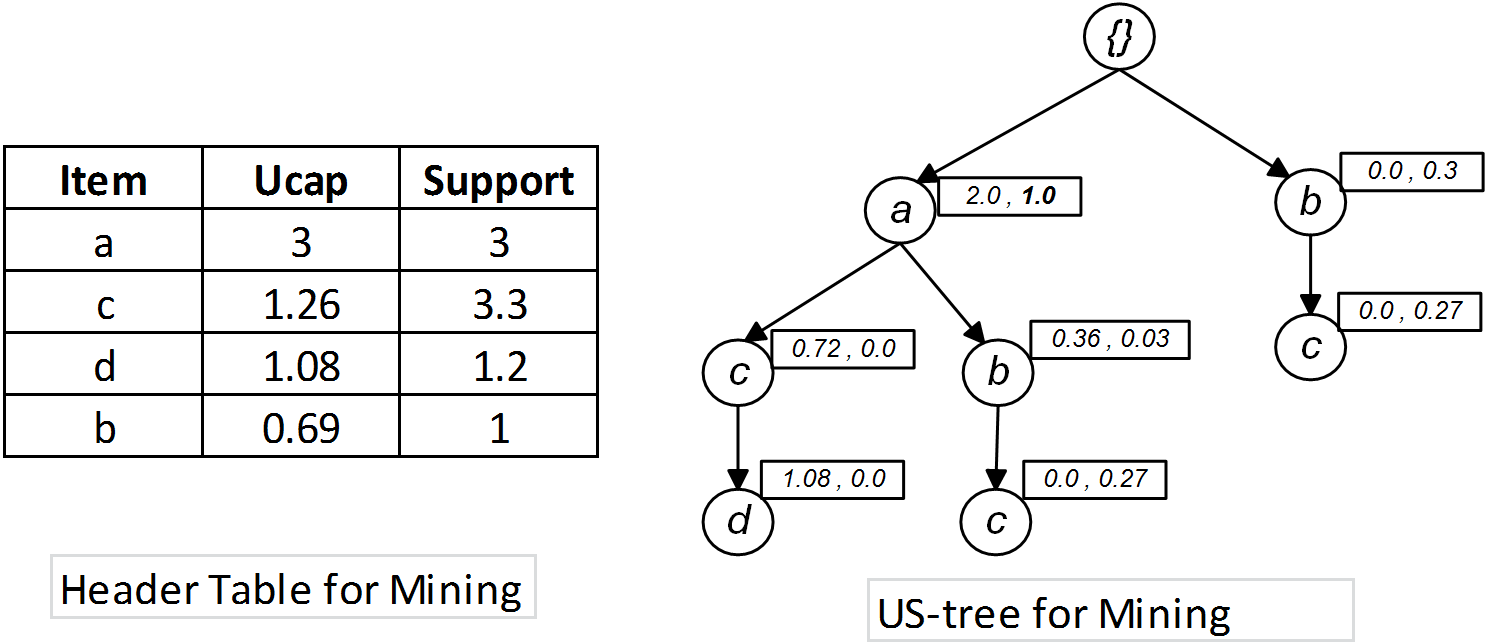
\includegraphics[width=0.9\textwidth]{visio/M_TREE}  
		\vspace*{-3mm}
	\caption{$\{e\}$-cond'l tree and its header table.S}
	\label{figure:E_COND_TREE_HEADER_TABLE}
    \end{minipage}%
    \begin{minipage}{0.55\linewidth}
    \centering
	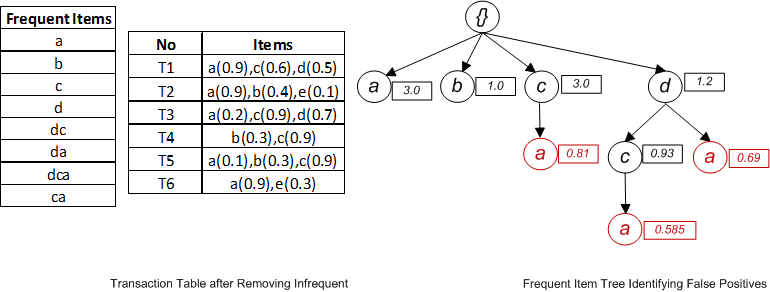
\includegraphics[width=0.9\textwidth]{visio/frequent_tree_final_ex}  
		\vspace*{-3mm}
	\caption{Frequent patterns and their frequent itemset trie with false positives.}
	\label{figure:FALSE_NEGATIVE}
    \end{minipage}
\end{figure*}

\subsubsection{US-tree Construction}

To capture the contents of transactions in a batch, our USFP-growth algorithm constructs a US-tree by inserting transactions from that batch into the the US-tree. Tree paths containing the same tree nodes (which represent items) are merged. By doing so, the resulting \mbox{US-tree} can be compact.
For example, to construct a \mbox{US-tree}, we examine $T_1 = \{a$:0.9, $c$:0.6, $d$:0.5, $e$:0.2\}, compute the $U^{cap}$ values for the four items as in Section~\ref{sec:prep}, and insert them into the US-tree. 
As a result, we get a tree path $\langle a$:0.9, $c$:0.54, $d$:0.45, $e$:0.18$\rangle$. 
Then, we examine $T_2 = \{a$:0.9, $b$:0.4, $e$:0.1\}, compute the $U^{cap}$ values for the three items:
$U^{cap}(a) = 0.9$, 
$U^{cap}(b) = 0.9 \times 0.4 = 0.36$, and
$U^{cap}(e) = 0.9 \times 0.1 = 0.09$.
We then try to insert new path $\langle a$:0.9, $b$:0.36, $e$:0.09$\rangle$ them into the US-tree. 
As this new path shares the common prefix $a$, the prefix of the two paths can be merged and nodes in the corresponding common prefix can be updated. Specifically, we merge and update the prefix value of $a$ to 0.9 + 0.9 = 1.8. So far, the only child of $a$ in the US-tree is $c$, we insert a path $\langle b$:0.36, $e$:0.09$\rangle$ as a child of $a$.
Similarly, we examine $T_3 = \{a$:0.2, $c$:0.9, $d$:0.7\}, compute the $U^{cap}$ values for the three items:
$U^{cap}(a) = 0.2$, 
$U^{cap}(c) = 0.2 \times 0.9 = 0.18$, and
$U^{cap}(d) = 0.9 \times 0.7 = 0.63$.
We then try to insert new path $\langle a$:0.2, $c$:0.18, $d$:0.63$\rangle$ them into the US-tree. 
As this new path shares the common prefix $\langle a, c, d\rangle$, the prefix of the two paths can be merged and nodes in the corresponding common prefix can be updated. Specifically, we merge and update the prefix value of $a$ to 1.8 + 0.2 = 2, that of $c$ to 0.54 + 0.18 = 0.72, and that of $d$ to 0.45 + 0.63 = 1.08. 

Afterwards, we process the second batch $B_2$ of transactions in a similar fashion, except that we store a second value for $U^{cap}$ in each node (in which its first value is the $U^{cap}$ value for batch $B_1$).
For example, we insert a new path $\langle b$:0,0.3, $c$:0,0.27$\rangle$ as a child of the root when processing $T_4 = \{b$:0.3, $c$:0.9\}. We merge and update the prefix values of $a$ to 2,0.1 and $b$ to 0.36,0.03, and insert $c$:0,0.27 as a child of $b$ when processing $T_5 = \{a$:0.1, $b$:0.3, $c$:0.9\}.
We merge and update the prefix values of $a$ to 2,0.1+0.9 = 2,1, and insert $e$:0,0.27 as a child of $a$ when processing $T_6 = \{a$:0.9, $e$:0.3\}. See Figure~\ref{figure:t1_6}.

As the window size is 2 batches, we delete transactions from the older batch $B_1$ to make room for the insertion of transactions in the newer batch $B_3$. To make this update efficient, we maintain a header table which contains the information for the oldest data, i.e., pointer points to the oldest data and can be found easily to slide the whole tree. After processing batch $B_3$, the US-tree is updated as shown in Figure~\ref{figure:t7_9}. Due to path sharing, the resulting tree is compact and memory-efficient. The tree can also be constructed in a time-efficient manner. When the tree is small, fewer conditional trees are generated, and thus reduce the mining time.

%      \begin{figure}[]
        \centering
            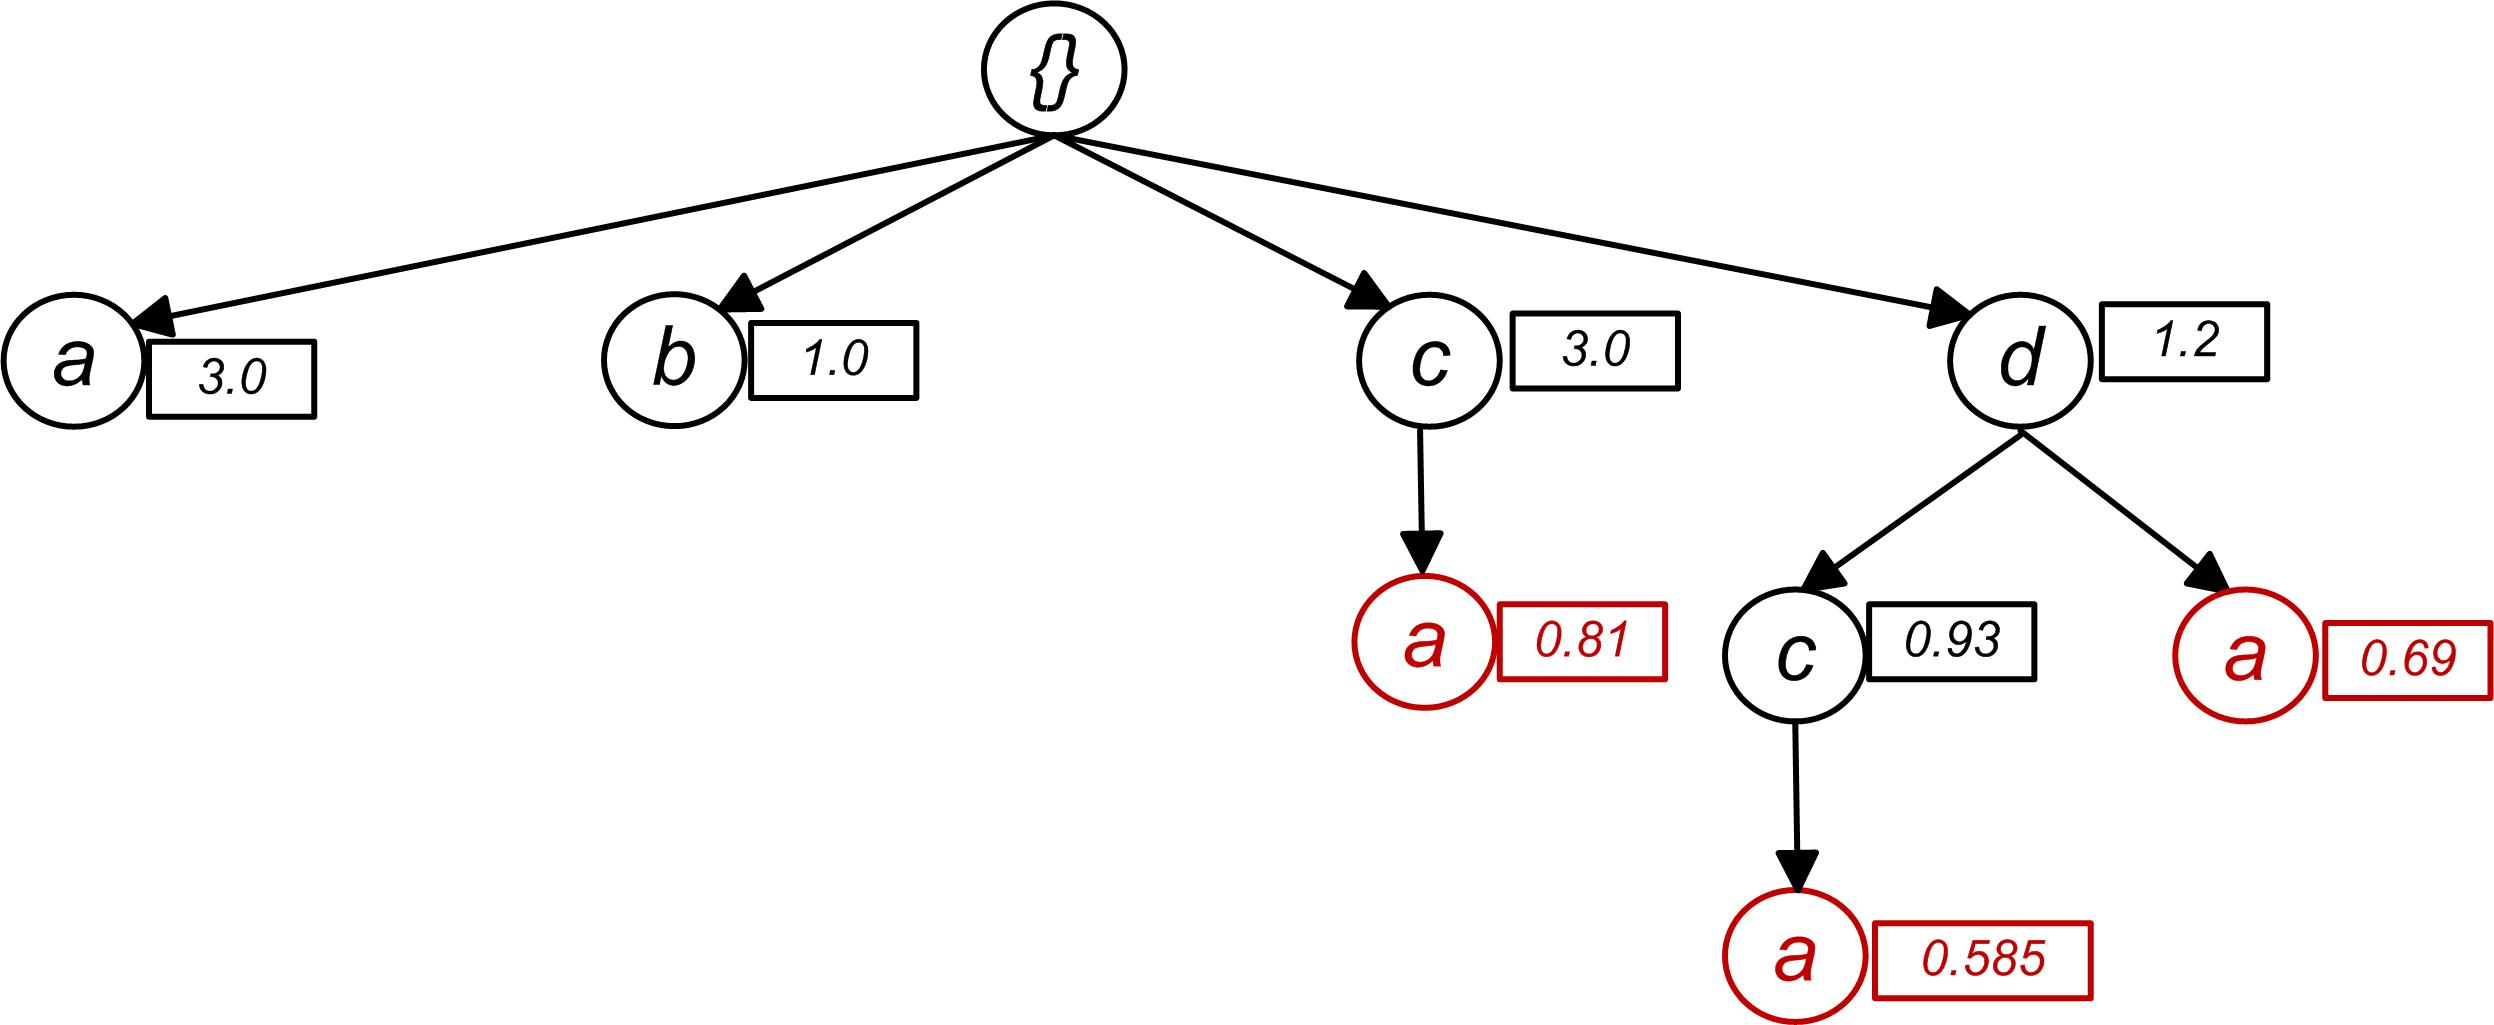
\includegraphics[width=.45\textwidth]{images/frequent_tree_final}
        \caption{Pattern Tree Identifying False Positives}
        \label{figure:frequent_patterns_final}
  \end{figure}



\begin{figure}
\begin{minipage}{0.15\textwidth}
  \centering
  
	\begin{center}
	\begin{tabular}{ |c| } 
 	\hline
 		FPs\\ \hline\hline
 		a \\ \hline
 		b \\ \hline
 		c \\ \hline
 		d \\ \hline
 		dc \\ \hline
 		da \\ \hline
 		dca \\ \hline
 		ca \\ \hline
\end{tabular}
\end{center}  


  \captionof{table}{Frequent Patterns}
\end{minipage}
\hfill
\begin{minipage}{0.30\textwidth}
  \centering
  
  \begin{center}
  \begin{tabular}{ |c|c| } 
  \hline
    No & Items \\ \hline\hline
    T\textsubscript{1} & \emph{a(0.9),c(0.6),d(0.5)}\\ \hline
    T\textsubscript{2}& \emph{a(0.9),b(0.4),e(0.1)}\\ \hline
    T\textsubscript{3}& \emph{a(0.2),c(0.9),d(0.7)}\\ \hline
    T\textsubscript{4}& \emph{b(0.3),c(0.9)}\\ \hline
    T\textsubscript{5}& \emph{a(0.1),b(0.3),c(0.9)} \\ \hline
    T\textsubscript{6} & \emph{a(0.9),e(0.3)
}\\ \hline
\end{tabular}
\end{center}  
  \captionof{table}{Transaction Table after Removing Infrequent}


\end{minipage}
\label{figure:frequent_patterns}
\end{figure}


\begin{figure*}[t]
	\begin{minipage}{0.24\linewidth}
		\centering
		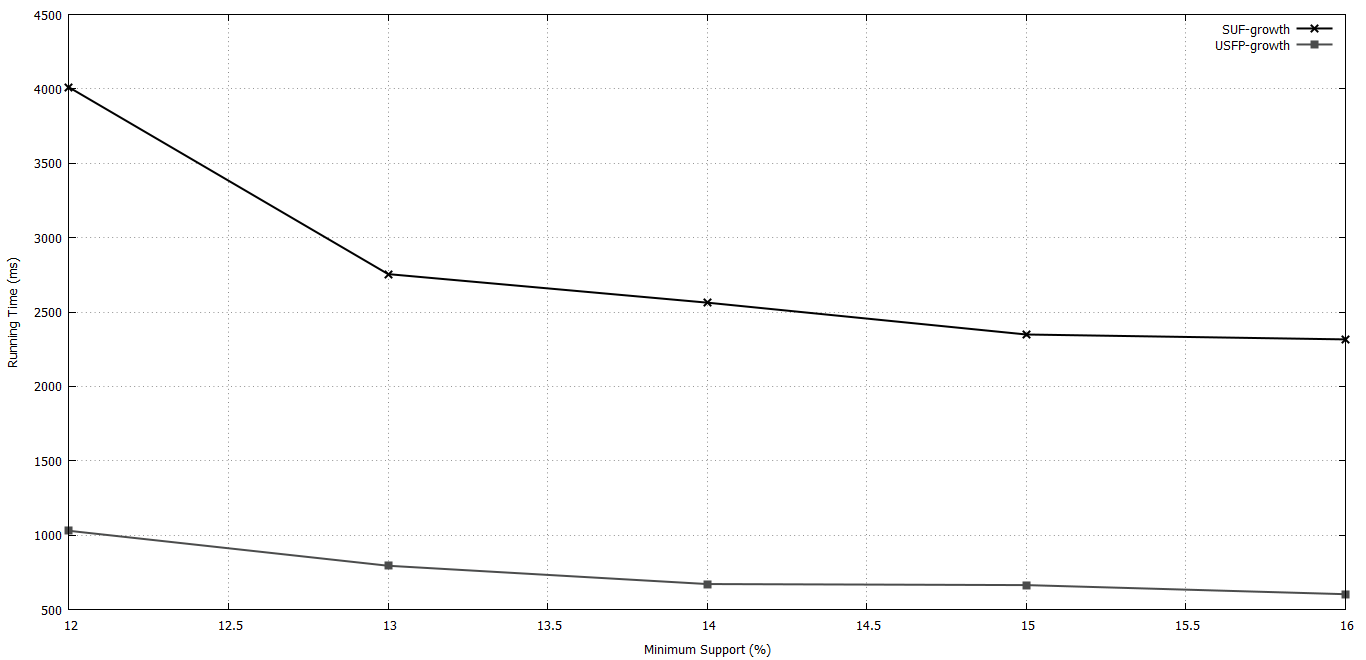
\includegraphics[width=\textwidth]{images/result/g_m_total}
		\vspace*{-7mm}
		\caption{Runtime for Mushroom.}
		\label{result:g_m_total}
	\end{minipage}%
    \begin{minipage}{0.24\linewidth}
		\centering
		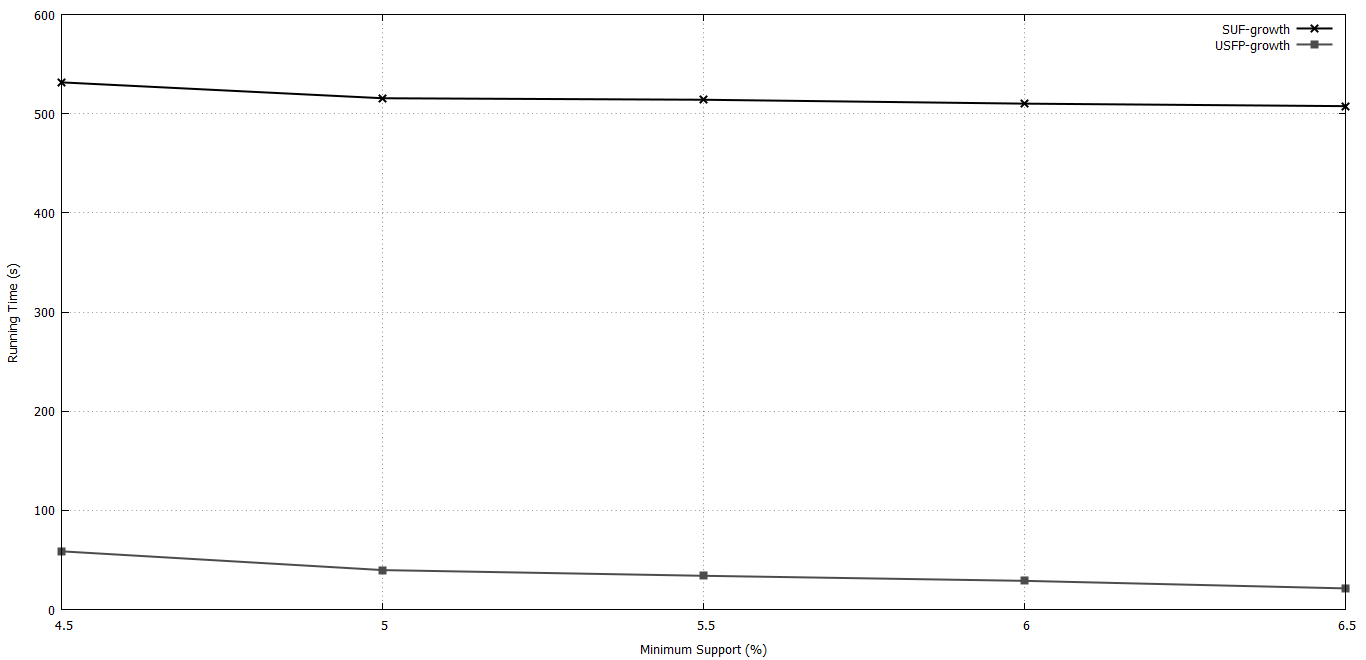
\includegraphics[width=\textwidth]{images/result/g_t10_total}
		\vspace*{-7mm}
		\caption{R'time for T40I10D100K.}
		\label{result:g_t10_total}
    \end{minipage}
	\begin{minipage}{0.24\linewidth}
		\centering
		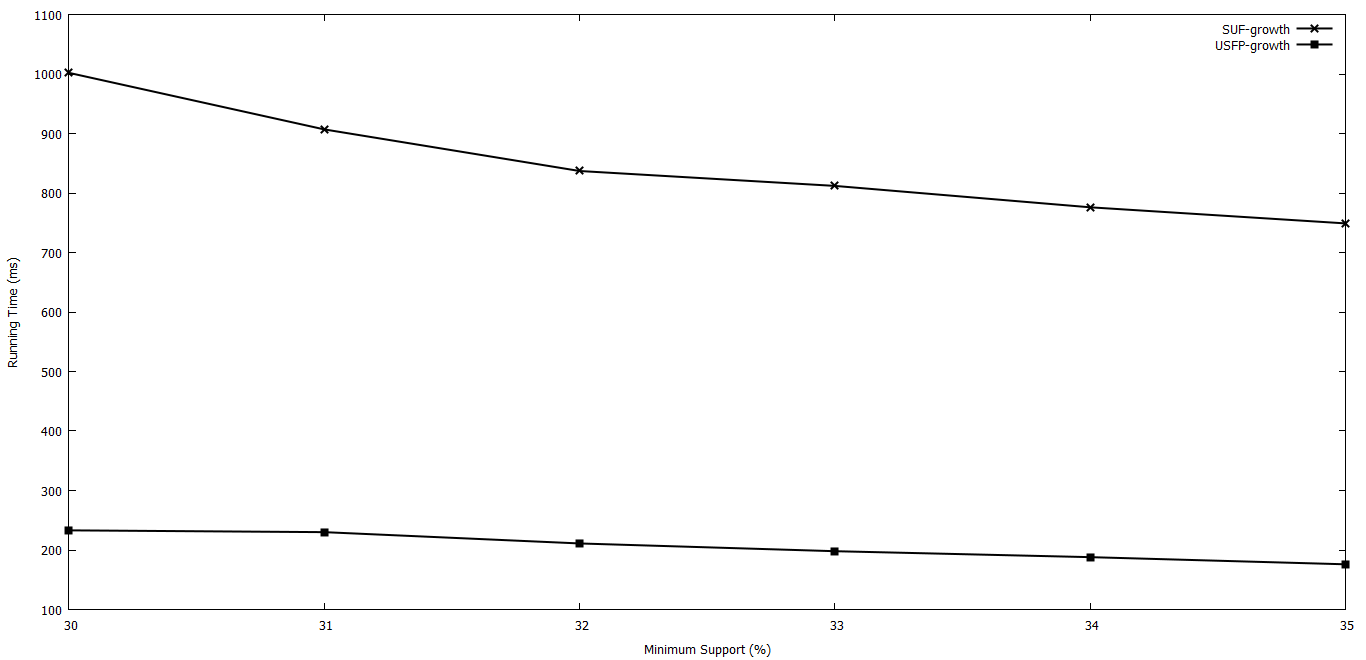
\includegraphics[width=\textwidth]{images/result/g_chess_total}
		\vspace*{-7mm}
		\caption{Runtime for Chess.}
		\label{result:g_chess_total}
	\end{minipage}%	
	\begin{minipage}{0.24\linewidth}
	   \centering
	   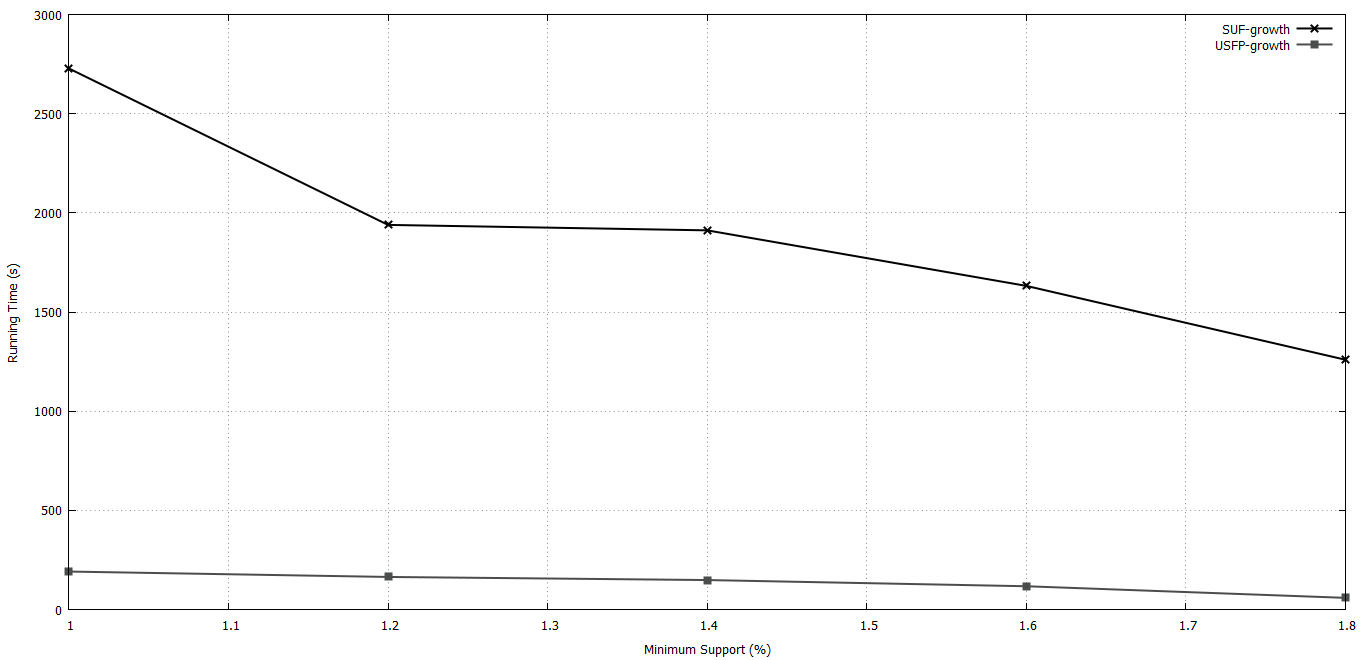
\includegraphics[width=\textwidth]{images/result/g_k_total}
		\vspace*{-7mm}
	   \caption{Runtime for Kosarak.}
	   \label{result:g_k_total}
	\end{minipage}
\end{figure*}

\subsubsection{Mining with USFP-growth}\label{sec:USFP}

As an extension to the tree-based algorithms (e.g., FP-growth, SUF-growth), our USFP-growth algorithm removes all the infrequent items (i.e., having support less than the user-specified minimum support {\it minsup} threshold). From the header table of \mbox{US-tree}, USFP-growth obtains information about the nodes that represent infrequent items. As we capture $U^{cap}$ (which can be served as an upper bound to support) in the US-tree, any nodes having $U^{cap} < {\it minsup}$ can be safely removed.
Then, USFP-growth constructs conditional tree starting from the lowest support holding node.
From the header table, we get the upper bounds to support of $a$=3, $c$=3.3, $d$=1.2, $b$=1, and $e$=0.6. Let {\it minsup}=0.9. Then, $e$ is infrequent, and it is guaranteed that no itemset containing $e$ will be frequent due to the downward closure property of frequent itemset. So, we remove the node $e$, and get the new tree (and its header table) as shown in Figure~\ref{figure:E_COND_TREE_HEADER_TABLE}. Here, we find all frequent singleton itemsets: $\{a\}, \{b\}, \{c\}$ and $\{d\}$. 

Next, we construct a conditional tree for each frequent singleton item, and mine frequent patterns from the tree. Again, items having total $U^{cap} < {\it minsup}$ are infrequent, and thus not consider in the conditional tree. In other words, we construct conditional trees from the item having the lowest total $U^{cap} \geq {\it minsup}$ to the item having highest total $U^{cap}$.
As $b$ with total $U^{cap} = 0.69 < {\it minsup}$, no conditional tree is constructed for $b$. Then, consider $d$ with total $U^{cap}$ = 1.08, which is contributed by the single path $\langle a, c, d\rangle$:1.08,0.
So, we create a $\{d\}$-conditional tree and update all the nodes in the tree. 
For this conditional tree (in Figure~\ref{figure:E_COND_TREE_HEADER_TABLE}), we find frequent $2^+$-itemsets $\{d,c\}, \{d,a\}$, and $\{d,c,a\}$.

Afterwards, we construct a $\{c\}$-conditional tree (Figure~\ref{figure:E_COND_TREE_HEADER_TABLE}) due to the three paths $\langle a,c\rangle$:0.72,0, $\langle a,b,c\rangle$:0,0.72 and $\langle b,c\rangle$:0,0.27. 
Knowing that $b$ having a total $U^{cap} < {\it minsup}$, $b$ is removed from the $\{c\}$-conditional tree and frequent \mbox{2-itemset} $\{c,a\}$ is found. 

We do not construct $\{c,a\}$- or $\{a\}$-conditional trees as they would be empty trees. When mining after $T_6$ in batch $B_2$, we found frequent patterns $\{a\}, \{b\}, \{c\}, \{d\}, \{d,c\}, \{d,a\}, \{d,c,a\}$ and $\{c, a\}$. As we found all patterns by using $U^{cap}$, it is guaranteed that there will be no false negatives. However, some false positives may exist among the mined frequent itemsets. 

\subsubsection{Reduction of false positives}

{\em False positives} are patterns that are returned by mining algorithms as frequent but are actually infrequent; {\em false negatives} are actually frequent patterns that are missed by mining algorithms.
With the use of $U^{cap}$ in the construction of US-trees, our USFP-growth algorithm may generate some false positives but no false negatives.

To eliminate false positives, we use two scans of transactions. In the first scan, we eliminate the infrequent \mbox{1-itemsets}. In the second scan, we update a frequent itemset trie with exact support so that false positives can be eliminated.
With the USFP-growth algorithm described in Section~\ref{sec:USFP}, $\{a\}, \{b\}, \{c\}, \{d\}, \{d,c\}, \{d,a\}, \{d,c,a\}$ and $\{c, a\}$ are returned. 
As checking whether an 1-itemset is frequent does not need $U^{cap}$, we can compute truly frequent 1-itemsets by the first scan. All four mined 1-itemsets $\{a\}, \{b\}, \{c\}$ and $\{d\}$ are truly frequent. 
With the second scan, mined $2^+$-itemsets are inserted into the frequent itemset trie. Any $2^+$-itemsets containing any infrequent \mbox{1-itemsets} are omitted. In our example, all the mined \mbox{$2^+$-itemsets} are kept in the trie. Then, by traversing the trie with {\it minsup}=0.9, paths with true support $< {\it minsup}$ (e.g., $\{c,a\}$:0.81, $\{d,c,a\}$:0.585 and $\{d,a\}$:0.69) are eliminated. Consequently, we return to the user only those truly frequent patterns (with their true support): $\{a\}$:3, $\{b\}$:1, $\{c\}$:3.3, $\{d\}$:1.2 and $\{d,c\}$:0.93.

\begin{figure}[t]
	\begin{minipage}{0.49\linewidth}
		\centering
		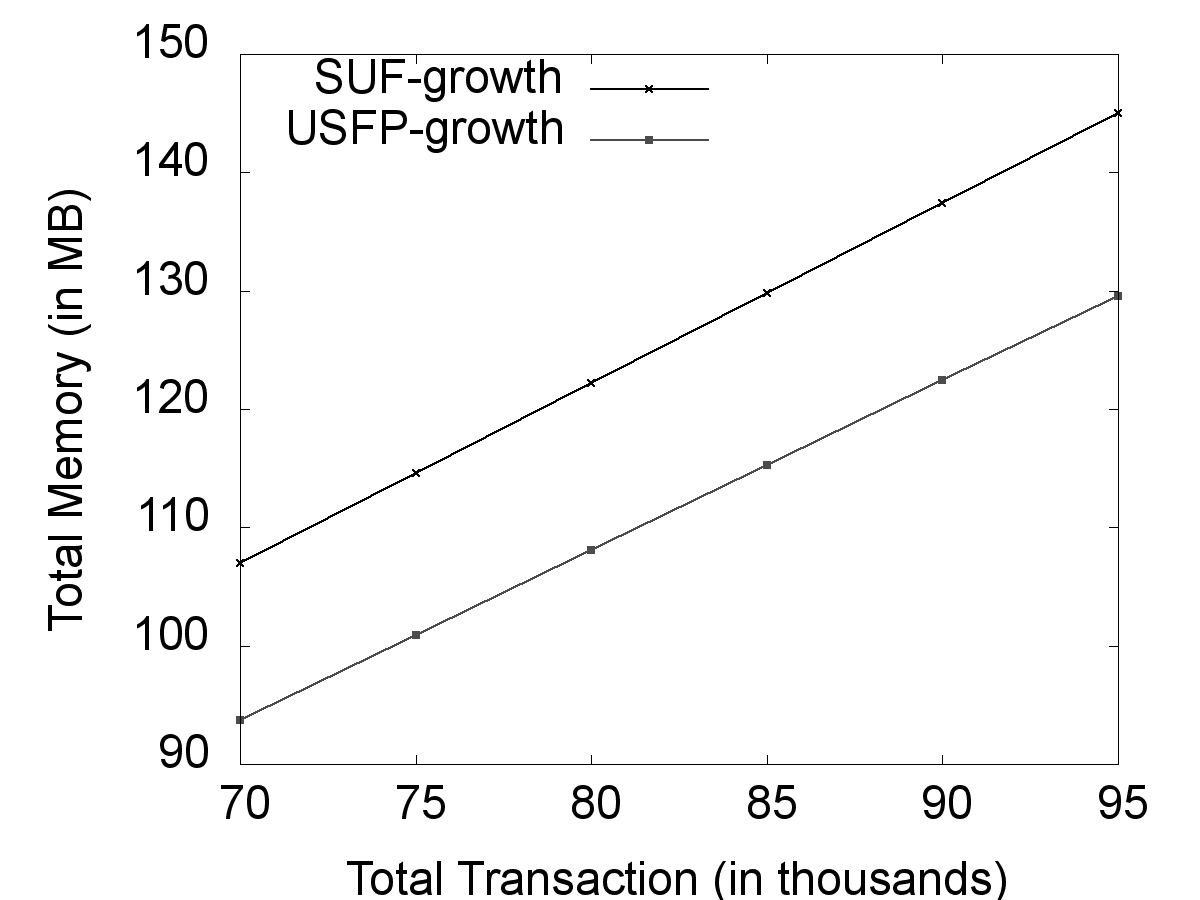
\includegraphics[width=\textwidth]{images/result/g_t10_memory_node}
		\caption{Memory Comparison for T40I10D100K}
		\label{result:g_t10_memory_node}
	\end{minipage}%
	\begin{minipage}{0.49\linewidth}
	   \centering
	   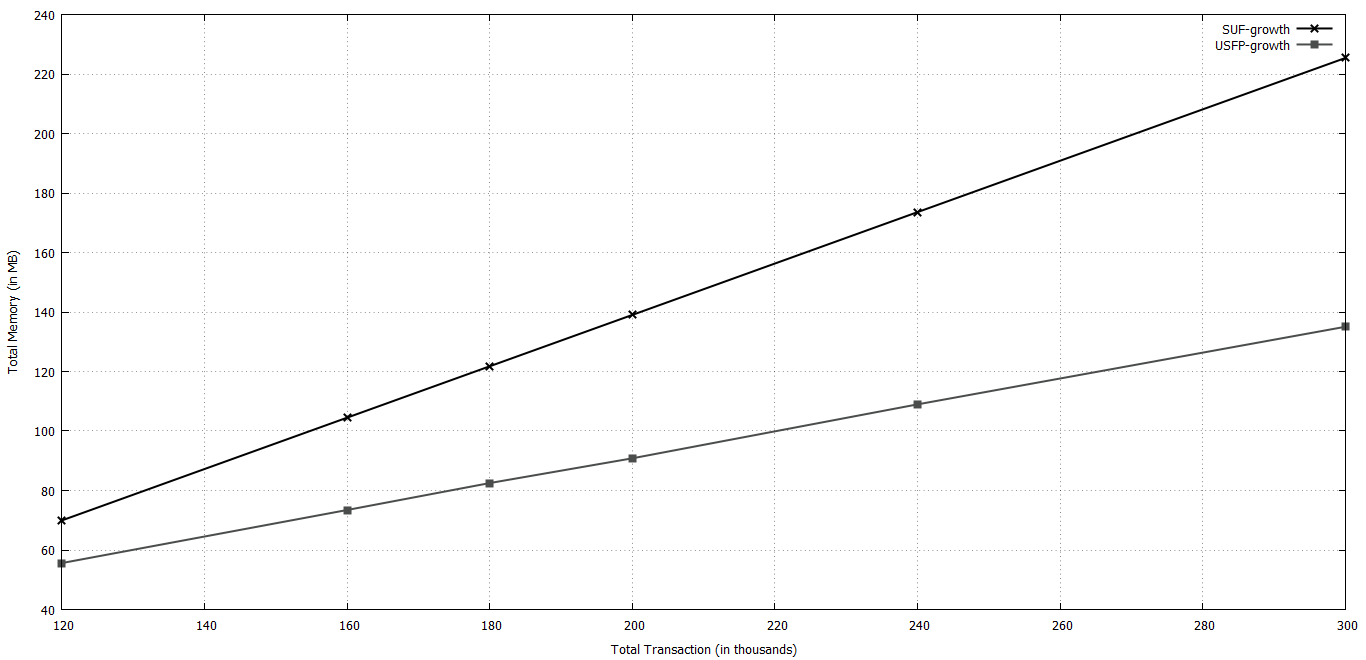
\includegraphics[width=\textwidth]{images/result/g_k_memory_node}
	   \caption{Memory Comparison for Kosarak}
	   \label{result:g_k_memory_node}
    \end{minipage}
\end{figure}

\section{Experimental Results}\label{Experiment}

We performed a number of simulations in our experiments on both synthetic datasets and real-life datasets, which are selected from the Frequent Itemset Mining Implementation (FIMI) Repository\footnote{http://fimi.ua.ac.be/data/}. Performance tests from our experiments show that the US-tree construction technique and \mbox{USFP-growth} mining algorithm can run on any uncertain stream datasets with any support threshold, window size, and batch size. Our experimental result shows that these techniques are much faster and scalable frequent pattern mining technique. We compared in all aspects to show the scalability, runtime efficiency and memory efficiency.
We collected data from the FIMI Repository, which contain precise (certain) data. Then, we used our own probabilistic tool and technique to generate the existential probability of each item of the each transaction of the dataset. Real-life data set actually follows Gaussian distribution (normal distribution). It actually says that in real life, extreme cases are the minimum and average cases are the maximum. We used \emph{Java pseudo-random} generator to produce the existential probability following Gaussian distribution. By assigning these probability values to each item, we have generated the uncertain database for all sample dataset. 
For the extensive experimental analysis, we have chosen the mushroom, T40I10D100K, chess, and Kosarak datasets. The reason we chose these two datasets is that the mushroom is a real-life dense dataset, whereas T40I10D100K is synthetic sparse dataset produced by a generator from the IBM Almaden Quest.

\subsection{Performance Comparison}

In this section, we compared our proposed approach with existing algorithm. We chose SUF-growth~\cite{DBLP:conf/icde/LeungH09} (most recent, latest state-of-the-arts algorithm) for comparison. This fits perfectly for uncertain stream data mining. \mbox{UF-streaming} was also designed for mining frequent patterns from uncertain stream but in~\cite{DBLP:conf/icde/LeungH09} it has been proved that in all criteria (runtime, memory and correctness) SUF-growth~\cite{DBLP:conf/icde/LeungH09} is better than UF-streaming~\cite{DBLP:conf/icde/LeungH09}. 

\subsubsection{Runtime Comparison}

Our proposed algorithm was evaluated based on runtime against existing algorithm using both dense and sparse datasets. For mushroom dataset, the total processing and runtime of proposed algorithm was compared with SUF-growth~\cite{DBLP:conf/icde/LeungH09} algorithm runtime. Figure~\ref{result:g_m_total} shows the result graph. As mushroom is a dense database we noticed significant gain. For dense characteristics, the constructed \emph{US-tree} is very much compact and moreover when mining compact tree, the mining time significantly decreases that affect the total time. Figure~\ref{result:g_t10_total} shows same comparison for T40I10D100K dataset. The graphs show that our algorithm works correctly for sparse dataset too. Figure~\ref{result:g_chess_total} shows runtime for chess dataset. Kosarak is very large and real-life web-click data set. This database is sparse and very much large. Figure~\ref{result:g_k_total} shows the superiority of our proposed algorithm with respect to runtime for varying thresholds.    

\subsubsection{Memory Comparison}

As our proposed \emph{US-tree} is capable to share more nodes than \emph{SUF-growth}, we receive more benefits in memory. The experimental result comply the fact. Figure~\ref{result:g_t10_memory_node} and Figure~\ref{result:g_k_memory_node} show the memory comparison on T40I10D100K and Kosarak datasets. The graph clearly shows that with the increase of total transaction in the tree gives the much more gain. On these sparse databases, it has been clearly shown that lot of memory optimization has been possible with our proposed algorithm.

For dense dataset (both real and synthetic) our approach is very efficient. For sparse dataset, this also gives us gain both in memory and runtime. The $U^{cap}$ value gives much more benefit to share nodes in the \emph{US-tree}. The compactness of \emph{US-tree} is noticeable. Mining compact \emph{US-tree} gives the main surprise in the runtime.

\section{Conclusions}\label{Conclusion}

In this paper, we have proposed a new sliding window based probabilistic strategy for finding frequent patterns from uncertain dynamic data. The strategy comprises of a new upper bound of existential probability, $U^{cap}$, a new compact data-structure, \emph{US-tree} and an efficient algorithm \emph{USFP-growth} that recursively mine frequent patterns from \emph{US-tree}. In our strategy, node sharing is possible more frequently and this makes the tree more compact and efficient. To handle the stream of data, we have segmented the whole transactions into batches and windows. Instead of keeping the support we have kept new meta-data based on $U^{cap}$ value that helps further mining. Our developed \emph{USFP-growth} mining algorithm efficiently removes unnecessary patterns from the tree earlier, which helps to improve correctness. Our comprehensive experimental analyses prove the supremacy of proposed algorithm with respect to runtime (efficiency), memory consumption (scalability). We also developed a frequent pattern tree which may later be used to mine closed patterns and maximal patterns.

\ifCLASSOPTIONcompsoc
  % The Computer Society usually uses the plural form
  \section*{Acknowledgments}
\else
  % regular IEEE prefers the singular form
  \section*{Acknowledgment}
\fi

%\footnotesize
This project is partially supported by the Natural Sciences and Engineering Research Council of Canada (NSERC).

%\bibliographystyle{IEEEtran}
%\bibliography{small_bibliography}
\begin{thebibliography}{10}
\setlength{\itemsep}{1mm}
%\providecommand{\url}[1]{#1}
%\csname url@samestyle\endcsname
%\providecommand{\newblock}{\relax}
%\providecommand{\bibinfo}[2]{#2}
%\providecommand{\BIBentrySTDinterwordspacing}{\spaceskip=0pt\relax}
%\providecommand{\BIBentryALTinterwordstretchfactor}{4}
%\providecommand{\BIBentryALTinterwordspacing}{\spaceskip=\fontdimen2\font plus
%\BIBentryALTinterwordstretchfactor\fontdimen3\font minus
%  \fontdimen4\font\relax}
%\providecommand{\BIBforeignlanguage}[2]{{%
%\expandafter\ifx\csname l@#1\endcsname\relax
%\typeout{** WARNING: IEEEtran.bst: No hyphenation pattern has been}%
%\typeout{** loaded for the language `#1'. Using the pattern for}%
%\typeout{** the default language instead.}%
%\else
%\language=\csname l@#1\endcsname
%\fi
%#2}}
%\providecommand{\BIBdecl}{\relax}
%\BIBdecl

\bibitem{ictai15FIM} C.~F. Ahmed, M. Samiullah, N. Lachiche, M. Kull, P.~A. Flach, ``Reframing in frequent pattern mining," in {\em IEEE ICTAI 2015}, pp.~799--806.

\bibitem{DBLP:conf/kdd/AggarwalLWW09}
C.~C. Aggarwal, Y.~Li, J.~Wang, and J.~Wang, ``Frequent pattern mining with
  uncertain data,'' in \emph{ACM KDD 2009}, pp.~29--38.

\bibitem{DBLP:conf/vldb/AgrawalS94}
R.~Agrawal and R.~Srikant, ``Fast algorithms for mining association rules in
  large databases,'' in \emph{VLDB 1994}, pp. 487--499.

\bibitem{tldks15} Alfredo Cuzzocrea, Fan Jiang, Carson K. Leung, Dacheng Liu, Aaron Peddle, Syed K. Tanbeer: Mining popular patterns: a novel mining problem and its application to static transactional databases and dynamic data streams. LNCS Transactions on Large-Scale Data- and Knowledge-Centered Systems (TLDKS) XXI (LNCS 9260), selected papers from DaWaK 2012: 115-139 (2015)

\bibitem{DBLP:conf/kdd/GadeWK04}
K.~Gade, J.~Wang, and G.~Karypis, ``Efficient closed pattern mining in the
  presence of tough block constraints,'' in \emph{ACM KDD 2004}, pp.~138--147.

\bibitem{DBLP:journals/datamine/HanPYM04}
J.~Han, J.~Pei, Y.~Yin, and R.~Mao, ``Mining frequent patterns without
  candidate generation: a frequent-pattern tree approach,'' \emph{Data Min.
  Knowl. Discov.}, 8(1), pp. 53--87, 2004.

\bibitem{ictai14} V. Kagklis, V.~S. Verykios, G. Tzimas, A.~K. Tsakalidis, ``An integer linear programming scheme to sanitize sensitive frequent itemsets," in {\em IEEE ICTAI 2014}, pp.~771--775.

\bibitem{DBLP:conf/icde/LeungH09}
C.~K. Leung and B.~Hao, ``Mining of frequent itemsets from streams of uncertain
  data,'' in \emph{IEEE ICDE 2009}, pp.~1663--1670.

\bibitem{www16} C.~K. Leung, R.~K. MacKinnon, and F. Jiang, ``Finding efficiencies in frequent pattern mining from big uncertain data," {\em World Wide Web}, 2016, doi:10.1007/s11280-016-0411-3

\bibitem{DBLP:conf/pakdd/LeungT13}
C.~K. Leung and S.~K. Tanbeer, ``PUF-tree: a compact tree structure for
  frequent pattern mining of uncertain data,'' in \emph{PAKDD 2013}, pp.~13--25.

\bibitem{ictai15udb} D.~M. Lyons, R.~C. Arkin, S. Jiang, D. Harrington, F. Tang, and P. Tang, ``Probabilistic verification of multi-robot missions in uncertain environments, in {\em IEEE ICTAI 2015}, pp.~56--63.

\bibitem{DBLP:journals/tkde/ZhaoYN14}
Z.~Zhao, D.~Yan, and W.~Ng, ``Mining probabilistically frequent sequential
  patterns in large uncertain databases,'' \emph{{IEEE} TKDE}, 26(5), pp. 1171--1184, 2014.
\end{thebibliography}
\end{document}


